This section specifies the software architecture requirements and the software architecture design
for the first level of granularity - the system as a whole. The output will be the high level software
architecture components, the infrastructure between them and the tactics used at the first level of
granularity to realize the quality requirements for the system.
Subsequent sections will focus on the software architecture requirements and design for these
high-level architectural components. Note that many of the architectural requirements (particularly
the quality requirements) will be propagated down to lower level architectural components.

\section{Architecture Requirements}
This section discusses the software architecture requirements around the 
required software infrastructure within which the application functionality is
to be developed. The purpose of this infrastructure is to address the
non-functional requirements. In particular the architecture requirements
specify.
\begin{itemize}
	\item the architectural responsibilities which need to be addressed
	\item the access and integration requirements for the system
	\item the quality requirements
	\item the architecture constraints specified by the client
\end{itemize}
\subsection{Access and Integration Requirements}
\subsubsection*{Access Channels}
At the first level of granularity we require one system access channel to
facilitate communication between the management and benchmark client service.

The benchmark client application or so-called \textit{monitor} application will upon
completion of the benchmarking jobs, need to report the results back to the
management system, which will need to process and persistent the results.
To accomplish this communication between these disparate systems, a messaging
platform will be used to facilitate communication.


\subsection{Quality Requirements}
\label{sec:overallQualityRequirement}
This section will specify the quality requirements at the highest level of
granularity. These requirements will propagate throughout the entire system
into every other component. Quality requirements that are specific to certain 
parts of the system will be discussed under the respective sections.

\subsubsection*{Flexibility}
The system should utilize dependency injection, open standard protocols and
open source library implementation's to allow the user to switch out any
realization of a technology with another.The system should use best software 
engineering practices as far as possible, to allow the system to be easily 
expanded upon by any member of the greater public community as this project is to
be released as an open source project.

\subsubsection*{Maintainability}
Among the most important quality requirements for the system is
maintainability. It should be easy to maintain the system in the future. To this end
\begin{itemize}
	\item Future developers should be able to easily understand the system,
	\item The technologies chosen for the system can be reasonably expected to be available for a long time
	\item Developers should be able to easily and relatively quickly
	\begin{itemize}
		\item Change aspects of the functionality the system provides, and
		\item Add new functionality to the system.
	\end{itemize}
  \item Configure a new monitor node to be able to fetch tasks and post its
    results to the system.
\end{itemize}

\subsubsection*{Scalability}
As this system is envisaged to be used in academia in very localized context,
a need for scalability doesn't exist.

\subsubsection*{Reliability}
The system must be reliable in terms of messages exchanged on the message platform
as we would want to avoid a situation where users results get lost in the
system and require users to possible run an expensive experiment a second
time.

Further more the results, experiment specifications and user uploaded artifacts
should be reliably sorted and retrieved, as these specifications all need to be
declared in academic research.

\subsubsection*{Security}
\label{sec:securityQualityRequirement}
As this system is a prototype, security is not a major concern. However security
should be kept in mind, as this is a software engineering best practice. However
full isolation on the monitor nodes and network isolation is outside of the scope
for this prototype.

A security requirement specified by the client is that of least privilege on 
the system as a whole. In this regard, the monitor nodes are only allowed to
communicate to the message platform, the management back end is only allowed to
communicate with the message platform and receive connections from the web interface.

\subsubsection*{Integrability}
The chosen message infrastructure and lower level components namely the
management system and monitor application should be integrable over a common
interface. Note however, as we are aiming for a loosely-coupled system, the 
management system will rather communicate with the monitor application than
integrate with it.

\subsubsection*{Deployability}
The system must be buildable from source and build scripts only.
The system must be deployable
\begin{itemize}
	\item on Linux servers,
	\item in environments using different message brokers for the
	enterprise message platform.
\end{itemize}

The system should ultimately be packaged as a series of Docker images which are
deployable as Docker containers installed on virtual or physical Linux servers.

\subsection{Architectural Responsibilities}
The architectural responsibilities of the messaging platform are shown in 
Figure \ref{fig:ESBResponsibilities}
\begin{figure}[H]
	\begin{center}
	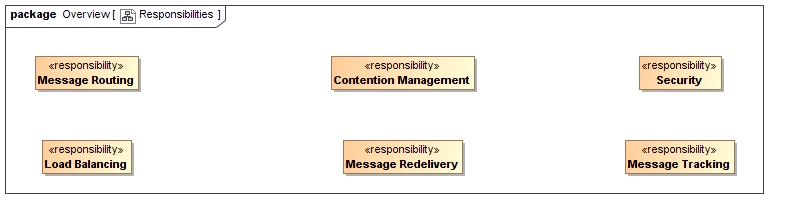
\includegraphics[scale=0.5]{../Diagrams and Charts/Overview/Responsibilities.jpg}
	\caption{The architectural responsibilities of the Messaging Platform}
	\label{fig:ESBResponsibilities}
	\end{center}
\end{figure}

\subsection{Architecture Constraints}
\label{sec:systemArchitecturalConstraints}
The chosen architecture was determined to best fulfill the non-functional
requirements for the system as well as the requirements set forth by the
client.
\begin{itemize}
	\item The architecture must be deployable on Linux servers
	\item All libraries, frameworks, programming languages and any other
	material of sort utilized within this project must be open-source.
	\item All libraries, frameworks, programming languages and any other
	material of sort used must be supported by open standards, have an 
	active and vibrant support community and should have an active 
	release cycle. 	
\end{itemize}

\subsection{Architecture Design}
\subsubsection{Frameworks and Technologies}
\paragraph*{Messaging Broker}
As the benchmark service is based on an messaging architecture,
the choice of which message platform to use is a critical decision. It was
determined that the Apache ActiveMQ will be used as the reference implementation. 

Apache ActiveMQ has a vibrant support community, supports various programming
languages, and has a very active release cycle, with the latest stable release
being version 5.13.1 released in February 2016, at this time of this writing.

Features of Apache ActiveMQ includes:
\begin{itemize}
	\item Spring Framework support
	\item Support J2EE servers
	\item Supports pluggable transport protocols
	\item Designed for high performance clustering and client-server communication
	\item Full support for Enterprise Integration Patterns
\end{itemize}

Other implementations considered:
\begin{itemize}
	\item Apache Apollo
	\item Apache Qpid
	\item Pivotal RabbitMQ
\end{itemize}

\subsubsection{Concepts and Constraints for Application Components}
ActiveMQ provides an implementation of a messaging architecture used to provide
integration between disparate business services.

Messaging architectures are commonly used to decouple business services from 
one another while providing reliable communication between these disparate 
systems. 
